NNs allow us to choose the feature maps in the model itself

\begin{center}
    \resizebox{0.6\linewidth}{!}{
    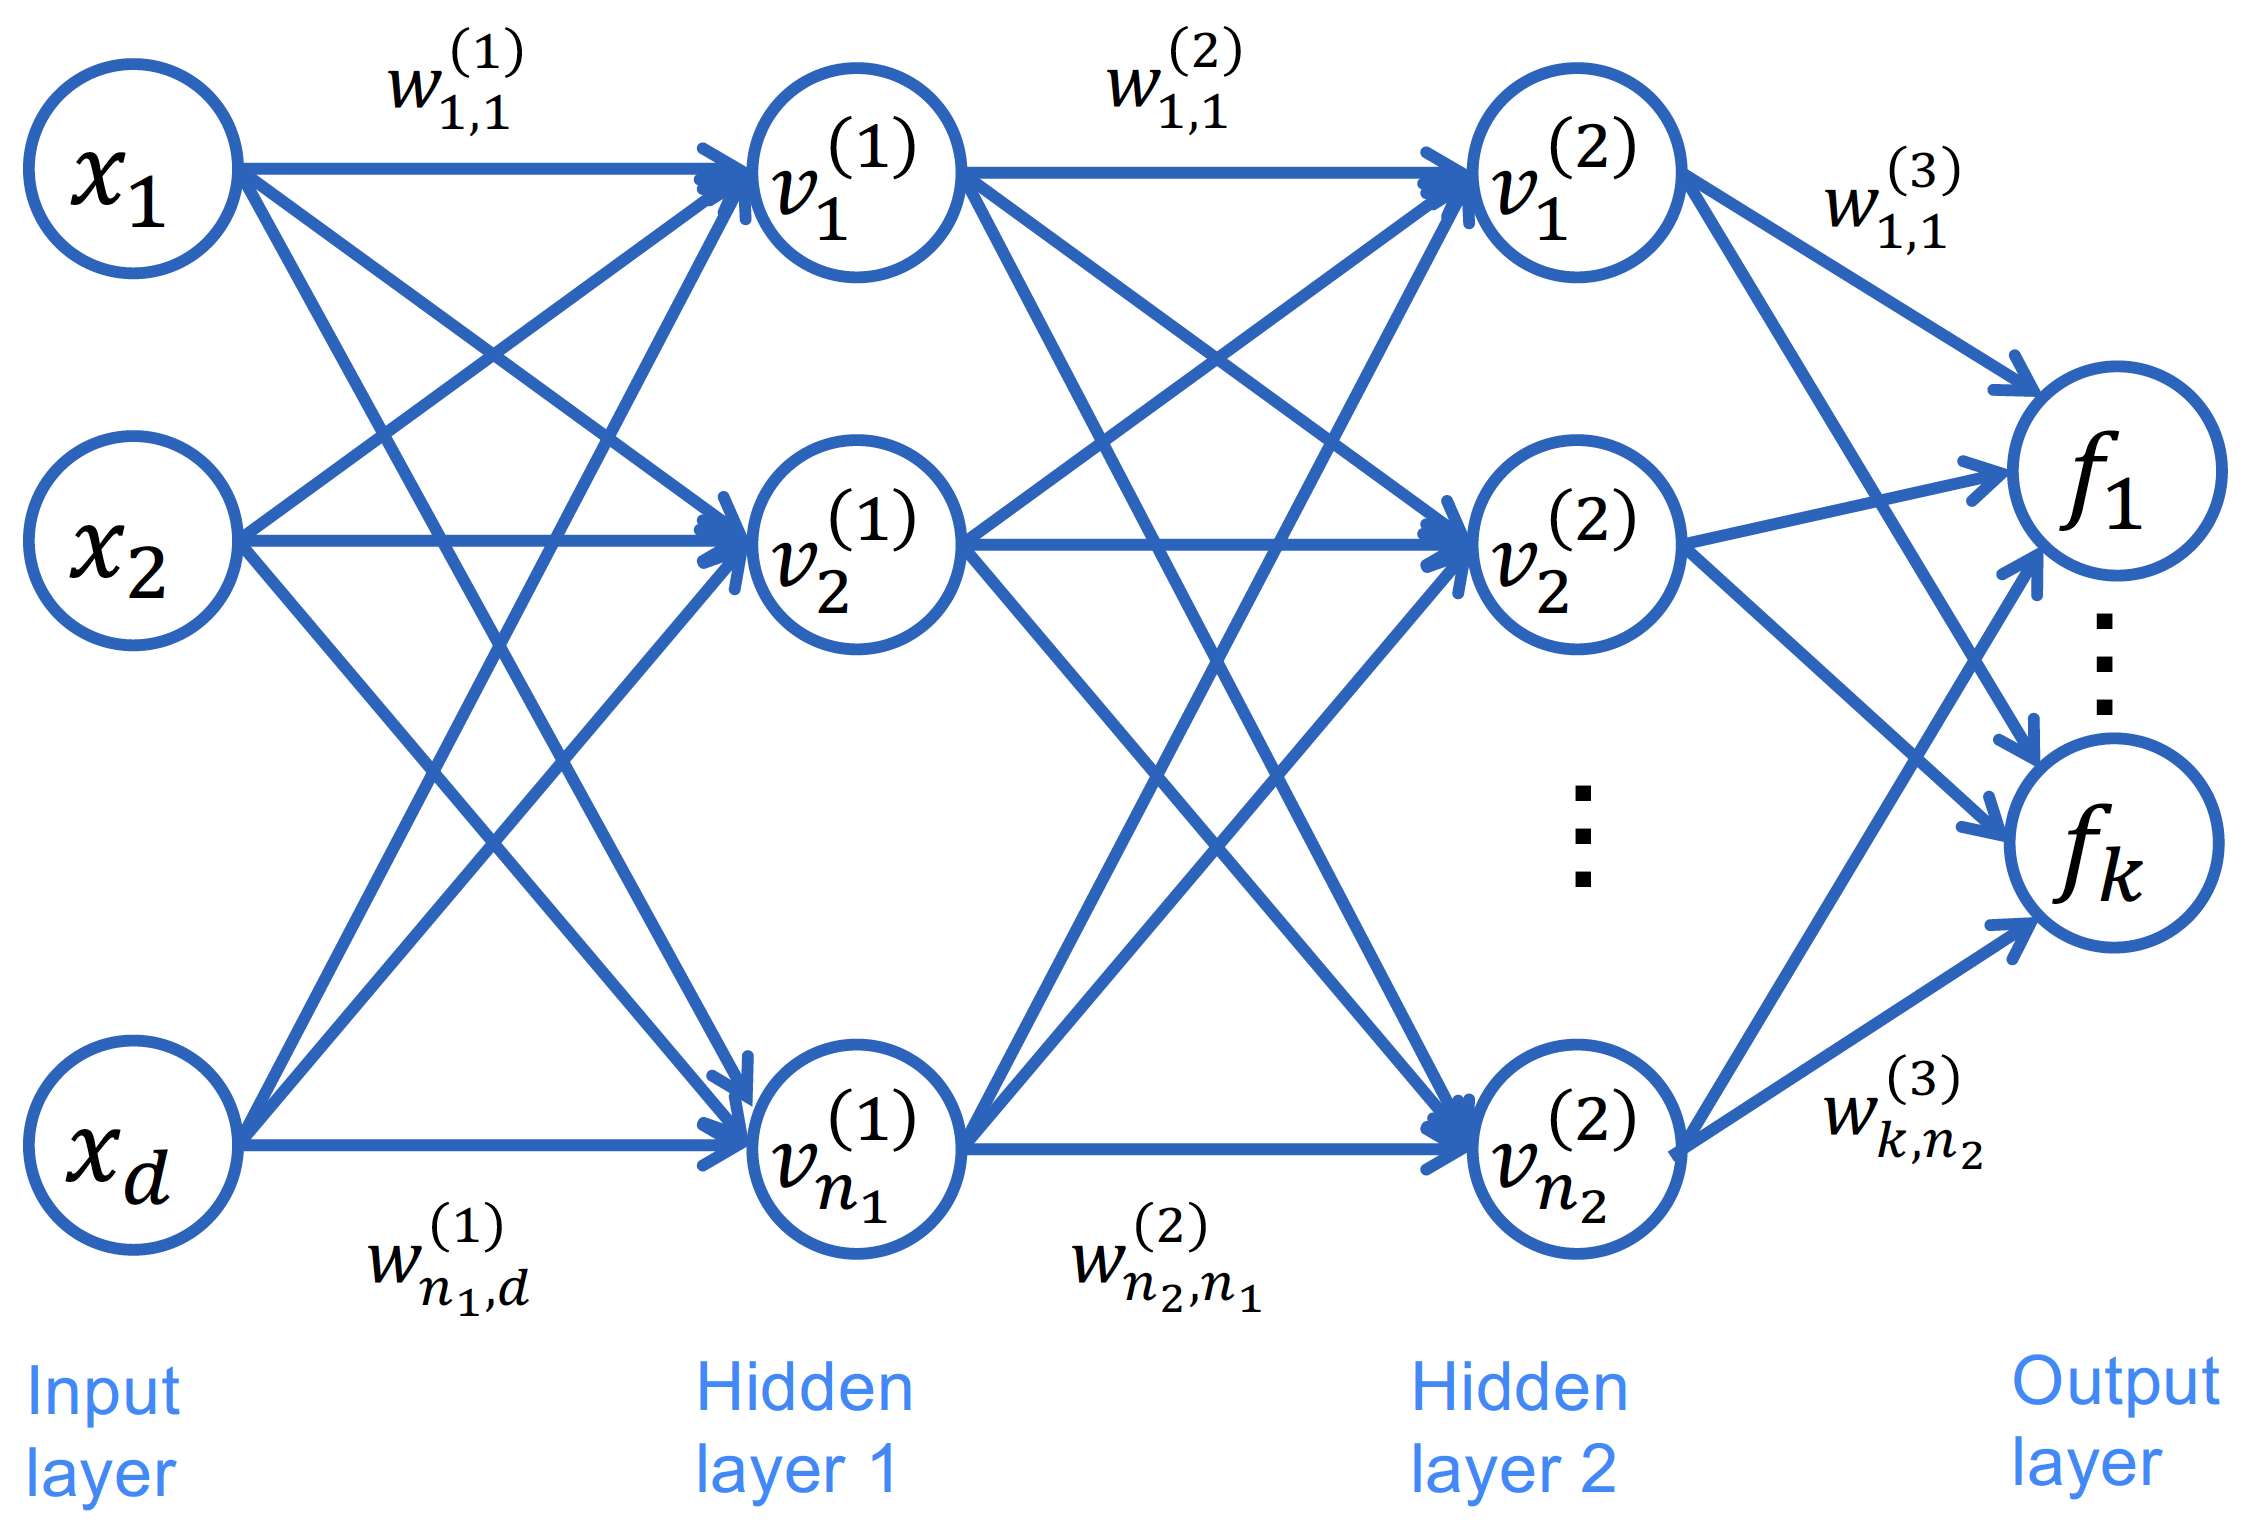
\includegraphics{images/NN.png}
    }
\end{center}

\begin{center}
    $z_1^{(1)} = \sum_{j=1}^d\omega_{1,j}^{(1)}x_j + \omega_{1,0}^{(1)}$\\
    $z_k^{(l)} = \sum_{j=1}^{n_{l-1}}\omega_{k,j}^{(l)}v_{j}^{(l-1)} + \omega_{k,j}^{(l)}$ \hspace{0.2cm} $v_l = \varphi(z_l)$
\end{center}
for $l = 1,..,L$ the number of layers

Vector notation:
\begin{center}
    $\boldsymbol{z}^{(l)} = \boldsymbol{W}^{(l)}\boldsymbol{v}^{(l-1)} + \boldsymbol{W}_0^{(l)}$\\
    $f(\boldsymbol{x}) = \boldsymbol{W}^{(L)}\boldsymbol{v}^{(L-1)}$\\
    where $\boldsymbol{v}^{(l)} = \left[\varphi(\boldsymbol{z}^{(l)};1)\right]$ $\varphi$ applied comp. wise
\end{center}

$\rightarrow$ optimize weights w.r.t. loss function (squared loss, cross-entropy etc.)

\begin{center}
    $l(\boldsymbol{W};\boldsymbol{x},y)= \sum_{i=1}^nl_i(\boldsymbol{W};\boldsymbol{x}_i,y_i)$
\end{center}
Universal approx. theorem: Any cont. fct can be approximated by a finite layered NN with sigmoidal act. function.

Weight decay reduces complexity
\subsection{Activation Functions}

A neural network with one hidden layer and nonlinear activation functions can approximate every continuous function.

\begin{itemize}
    \item Sigmoid
    \item Relu
    \item Relu Variants
\end{itemize}
\subsection{Backpropagation}

Can reuse computations from \color{NavyBlue} forward propagation \color{black} and from \color{Green} layer $l_{i+1}$ ... \color{black} to \color{Red} compute \color{black} $W^{(i)}$ 

\begin{center}
    $(\nabla_{W^{(i)}}l)^T  = \color{Green}\underbrace{\frac{\partial l}{\partial f}}_{\delta{(L)}}\frac{\partial f}{\partial z^{(L-1)}}\frac{\partial z^{(L-1)}}{\partial z^{(L-2)}}...\color{Red} \frac{\partial z^{(i+1)}}{\partial z^{(i)}}\color{NavyBlue}\underbrace{\frac{\partial z^{(i)}}{\partial W^{(i)}}}_{v^{(i-1)}}$\\
    $\nabla_{W^{(l)}}l = \boldsymbol{\delta}^{(l)}\boldsymbol{v}^{(l-1)}$, $\boldsymbol{\delta}^{(l)} = diag(\varphi'(z^{(l)})W^{(l+1)})\boldsymbol{\delta}^{(l)}$\\
    $\omega^{(t+1)}_{L-l} \leftarrow \omega^{(t)} - \eta \frac{\partial l}{\omega_{L-l}}$
\end{center}
\textbf{Note} usually minibatches are used for cum. weight updates.

Runtime grows linearly with num of params in feed forward

\textbf{Modifications}:
\begin{center}
    Momentum: initialize $d = 0$\\
    $\boldsymbol{d} \leftarrow m*\boldsymbol{d} + \eta_t\nabla_Wl(\boldsymbol{W};\boldsymbol{x},y)$\\
    $W \leftarrow W - \boldsymbol{d}$
\end{center}


\subsection{Vanishing / Exploding Gradient}

Potential reasons:
\begin{itemize}
    \item $||\delta^{(i)}|| \rightarrow 0 | \infty$ or $||v^{(i)}|| \rightarrow 0 | \infty$
    \item Certain act. fct. like e.g. Relu (no saturation) can help avoid $\delta \rightarrow 0$
    \item Note $\delta$ only depends on $\varphi'$ while v depends on $\varphi$
    \item Helps to standardize input and / or use batch normalization
    \item Weight initialization matters as weight opt. is generally a non-convex problem
\end{itemize}



\subsection{Regularization in NNs}

Reg. term in loss fct., early stopping, dropout or data augmentation

\textbf{Batch norm.} Normalize unit activations for a laye:
\begin{itemize}
    \item $\mu_s = \frac{1}{|S|}\sum_{i\in S}v_i$
    \item $\sigma_S^2 = \frac{1}{|S|}\sum{i\in S}(v_i - \mu_S)^2$
    \item $\hat{v}_i = \frac{v_i - \mu_S}{\sqrt{\sigma_S^2} + \epsilon}$
    \item Scale and shift: $\bar{v}_i = \gamma\hat{v}_i + \beta$, $\gamma,\beta$ given params.
\end{itemize}
Speeds up and stabilizes training. Solves covariate shift, reduces importance of weight init. Introduces exploding gradients. Mild reg. effect because of "random" batch size.
\subsection{Convolutional Neural Networks}

Unfeasible to fully connect vectorized images due to number of parameters.

\begin{itemize}
    \item Invariant regarding shifts, scale and rotation
    \item Updates still through backpropagation
\end{itemize}

\textbf{Dimension of image after CNN layer}
image: n x n, m kernels of size k*k, stride s, padding p:

\begin{center}
    $l = \frac{n + 2p -k}{s} + 1$
\end{center}

\textbf{(Max)Pooling}

Strongly reduces number of parameters

\subsection{Residual NNs}

\begin{itemize}
    \item Helps avoid vanishing gradients
    \item Allows for very deep NNs (1000+ layers)
\end{itemize}
